%! Author = biebl
%! Date = 02.05.2023


\chapter{Technische Details}\label{ch:technische-details}
In diesem Kapitel soll es um die technischen Details von Vue.js gehen.
Es wird ein Überblick gezeigt von verschiedenen in Vue.js vorhandenen Elementen
und es wird auf diese anhand von Beispielen genauer eingegangen.
Die Betrachtung bezieht sich auf Vue 3.
Aufgrund der Kürze der Arbeit und des Funktionsumfangs von Vue.js ist es nicht mögliche alle Features abzudecken.
Das Kapitel dient dazu, dem Leser einen ersten Eindruck von Vue.js zu geben.


\section{Options API vs. Composition API}\label{sec:options-api-and-composition-api}
Vue.js organisiert einzelne Komponenten als \emph{Single-File Components (SFC)},
die im HTML-ähnlichen Dateiformat mit der Dateiendung \texttt{.vue} vorliegen.
In einem SFC werden Aussehen, Struktur und Logik einer Komponente gebündelt, bestehend aus HTML-, CSS- und JavaScript-Elementen.
Für den Aufbau einer solchen SFC gibt es seit Vue 3 zwei verschiedene Möglichkeiten.
Zum einen gibt es die \emph{Options API} und zum anderen die \emph{Composition API}. \cite{vueIntroduction}

\subsection*{Options API}
Die länger vorhandene Variante ist die Options API.
Bei der Options API wird für die Komponente ein JavaScript Objekt angelegt.
Das Objekt kann verschiedene Optionen enthalten, darunter \texttt{data} für Daten, \texttt{methods} für Methoden und auch Lifecycle-hooks wie \texttt{mounted}.
\cite{vueIntroduction}

\subsection*{Composition API}
Die Composition API kam mit Vue 3 hinzu und wurde später für Vue 2 nachgereicht \cite{vueFAQ}.
Bei der Verwendung der Composition API werden in einem \texttt{import}-Statement
die benötigten API-Features wie zum Beispiel Lifecycle-hooks angegeben.
Der Code bei Verwendung der Composition API wird in der Regel zwischen einem \texttt{<script setup>} Tag verwendet.
Durch die Verwendung des Tags wird zur Compilezeit eine Transformation durchgeführt,
die es ermöglicht, die Composition API mit weniger redundantem Code zu nutzen.
Somit ist es möglich, Variablen und Funktionen direkt im Template zu verwenden.
\cite{vueIntroduction}

\subsection*{Gegenüberstellung}

\begin{minipage}[t]{.45\textwidth}
    \begin{lstlisting}[caption={Options API},language=javascript, label={lst:OptionsAPI}]
<script>
export default {
  // reactive state
  data() {
    return {
     wasPressed : false
    }
  },

  // functions that mutate state and trigger updates
  methods: {
    setStatus() {
      this.wasPressed = true
    }
  },

  // lifecycle hooks
  mounted() {
    console.log(`mounted`)
  },

  update(){
    console.log(`update`)
  },

  unmounted(){
    console.log(`unmounted`)
  }
}
</script>

<template>
  <button @click="setStatus">Button was Pressed: {{ wasPressed }}</button>
</template>
    \end{lstlisting}
\end{minipage}%
\hspace{1cm}
\begin{minipage}[t]{.5\textwidth}
    \begin{lstlisting}[caption={Composition API},language=javascript, label={lst:CompositionAPI}]
<script setup>
import { ref, onMounted, onUpdated, onUnmounted } from 'vue'

// reactive state
const wasPressed = ref(false)

// functions that mutate state and trigger updates
function setStatus() {
  wasPressed.value = true;
}

// lifecycle hooks
onMounted(() => {
   console.log(`mounted`)
})

onUpdated(() => {
   console.log(`updated`)
})

 onUnmounted(() => {
   console.log(`unmounted`)
})

</script>

<template>
  <button @click="setStatus">Button was Pressed: {{ wasPressed }}</button>
</template>
    \end{lstlisting}
\end{minipage}

In Vue.js können beide APIs ohne Einschränkung genutzt werden.
Hier sind zwei gleichwertige Beispiele in \ref{lst:OptionsAPI} und \ref{lst:CompositionAPI} dargestellt,
die jeweils mit einer der APIs implementiert wurden.
Es werden Veränderungen im Lifecycle auf der Konsole ausgegeben und es wird festgehalten, ob ein Button gedrückt wurde.
Für Anfänger mit ersten Erfahrungen in Objektorientierung wird die Options API empfohlen.
Ansonsten sollte die Options API nur bei weniger komplexen Kleinprojekten genutzt werden.
Für größere Projekte wird die Composition API empfohlen. \cite{vueIntroduction}

\subsection*{Fazit zu Options API vs. Composition API}
Die Composition API ist deutlich übersichtlicher, strukturierter und spart redundanz im Code.
Auch bei weniger komplexen Kleinprojekten könnte sich die Options API als ungeeignet erweisen,
da unvorhergesehene Größenänderungen dazu führen können,
dass die wartbare Composition API die bessere Wahl ist.
Die Composition API ist der Options API vorzuziehen.


\section{Direktiven in Vue.js}\label{sec:direktiven-in-vue.js}
Direktiven beschreiben ein gewünschtes Verhalten in der View.
In Vue.js beginnen diese Direktiven mit \texttt{v-}.
Vue.js bietet einige vordefinierte Direktiven wie \texttt{v-for}, \texttt{v-if}, \texttt{v-else}, \texttt{v-show}, \texttt{v-on}, \texttt{v-slot}, \texttt{v-bind}
und \texttt{v-model}, bietet aber auch die Möglichkeit, eigene Direktiven zu erstellen. \cite[S. 10]{steyer2019}
\\
Es wird sich auf eine Auswahl der vordefinierten Direktiven beschränkt.
Eine Liste aller Direktiven\footnote{\url{https://vuejs.org/api/built-in-directives.html}}
und wie man eigene Direktiven\footnote{\url{https://vuejs.org/guide/reusability/custom-directives.html}}
erstellt, ist in der Dokumentation von Vue.js zu finden.
Auf Direktiven zur Datenbindung wird an passenderer Stelle in Abschnitt \ref{sec:datenbindung-in-vue.js} eingegangen.


\subsection*{v-for}
\texttt{v-for} funktioniert wie eine foreach-Schleife.
Die \texttt{v-for}-Direktive ermöglicht es über eine Sammlung von Werten zu iterieren und die Daten in der View zu nutzen.
Erlaubte Datentypen sind \texttt{Array}, \texttt{Object}, \texttt{number}, \texttt{string} und solche, die das Interface \texttt{Iterable} implementieren. \cite{vueDirectives}
\begin{lstlisting}[caption={\texttt{v-for}-Direktive},language=html, label={lst:v-for}]
<div v-for="element in list">
  {{ element.value }}
</div>
\end{lstlisting}

%\newpage

\subsection*{v-if}
Die Direktive \texttt{v-if} ähnelt in der Funktionsweise einem if-Statement in der Programmierung.
\texttt{v-if} prüft anhand des übergebenen Wahrheitswerts, ob ein HTML-Element angezeigt werden soll.
Mit der Verwendung von \texttt{v-if} können Alternativen mit \texttt{v-else} für den Fall, dass die Bedingung nicht erfüllt ist,
oder mit \texttt{v-else-if} für eine bedingte Alternative ergänzt werden.
Entsprechend dem Wahrheitswert werden dann die Alternativen angezeigt. \cite{vueDirectives}
\begin{lstlisting}[caption={\texttt{v-if}-Direktive},language=html, label={lst:v-if}]
<div v-if="condition">
  condition is true
</div>
<div v-else-if="anotherCondition">
  anotherCondition is true
</div>
<div v-else>
  condition and anotherCondition are false
</div>
\end{lstlisting}

\subsection*{v-on}
Mit der \texttt{v-on}-Direktive wird ein Event-Listener an das HTML-Element gebunden.
Die Direktive erhält als Argument das Event, auf das der Listener reagieren soll,
sowie die darauf auszuführende Aktion.
Als Kurzform von \texttt{v-on} ist auch \texttt{@} möglich.
Mit \texttt{\$event} ist es möglich Eventeigenschaften weiter zugeben.
Darüber hinaus gibt es noch Modifier, die das zu erwartende Event präzisieren. \cite{vueDirectives}
\begin{lstlisting}[caption={\texttt{v-on}-Direktive},language=html, label={lst:v-on}]
<button v-on:click="buttonClicked"></button>
<button @click="buttonClickedButShortHand"></button>
<button v-on:click.right="buttonRightClicked"></button>
\end{lstlisting}

%\newpage


\section{Komponenten in Vue.js}\label{sec:komponenten-in-vue.js}
Komponenten sind wiederverwendbare Bausteine.
Die Komponenten können beliebig oft in der View verwendet werden und im Model unabhängig angesteuert werden.
Vue.js bietet die Möglichkeit, Komponenten selbst aus HTML, CSS, sowie JavaScript zu definieren und sie später mit einem
selbst  definierten HTML-Tag anzusteuern. \cite[S. 11-12]{steyer2019}
\\
Wie in Abschnitt \ref{sec:options-api-and-composition-api} bereits erwähnt, werden in Vue.js Komponenten normalerweise als SFC geschrieben.
Eine Komponente kann wie in Abschnitt \ref{sec:options-api-and-composition-api} erwähnt mit Composition API oder Options API
erstellt werden.
Alternativ kann man die Komponente als JavaScript Objekt erstellen, um den Build-Schritt zu umgehen (siehe Listing \ref{lst:Komponente als JavaScript-Objekt}).
Eine Komponente kann dann mit einem Alias im Script-Teile einer anderen Komponente importiert werden und muss dort noch als Komponente
registriert werden.
Nach dem Registrieren kann der Alias als Tag für die importierte Komponente verwendet werden. \cite{vueComponents}

\newpage

\begin{lstlisting}[caption={Komponente als JavaScript Objekt},language=javascript,label={lst:Komponente als JavaScript-Objekt}]
export default {
  data() {
    return {
     wasPressed : false
    }
  },
  template:`<button @click="setStatus">Button was Pressed: {{ wasPressed }}</button>`
}
\end{lstlisting}


\begin{lstlisting}[caption={Verwendung einer Komponente},language=javascript,label={lst:Verwendung einer Komponente}]
<script>

import ButtonStatusChecker from './ButtonStatusChecker.vue' //import of component

export default {
  components: {
    ButtonStatusChecker //component registration
  }
}
</script>

<template>
  <ButtonStatusChecker /> //using component
</template>
\end{lstlisting}

Neben der lokalen Registrierung existiert die Möglichkeit eine Komponente global
zu registrieren, um sie nicht bei jeder Verwendung in einer anderen Komponente
extra importieren und registrieren zu müssen.
Die globale Registrierung ist mit Aufruf der \texttt{component()}-Methode der App-Instanz möglich.
Der \texttt{component()}-Methode wird dann der Alias und die importierte \texttt{.vue}-Datei übergeben.
Alternativ kann auch die Implementierung beim Aufruf direkt übergeben werden. \cite{vueComponentsRegistration}

%\newpage

\begin{lstlisting}[caption={Globale Registrierung einer Komponente},language=javascript,label={lst:Globale Registrierung}]
import { createApp } from 'vue'
import ButtonStatusChecker from './ButtonStatusChecker.vue'
const app = createApp({})
app.component('ButtonStatusChecker', ButtonStatusChecker)
\end{lstlisting}


Um Daten an eine Komponente zu übergeben, gibt es die \texttt{props}-Option beim Erstellen einer Komponente.
Das \texttt{props}-Attribut erhält einen Namen, über die es dann später in
HTML angesteuert werden kann. \cite{vueComponents}

\newpage

\begin{lstlisting}[caption={Erstellung eines \texttt{props}},language=javascript,label={lst:Erstellung eines props}]
<script>
export default {
  props: ['text']
}
</script>

<template>
  <p>{{ text }}<p>
</template>
\end{lstlisting}

\begin{lstlisting}[caption={Nutzung eines \texttt{props}},language=javascript,label={lst:Nutzung eines props}]
<Paragraph text="Hallo Welt" />
\end{lstlisting}

Abgesehen von den bereits aufgezählten Features, bietet Vue.js für Komponenten weitere Features wie die Möglichkeit auf Events zu reagieren,
die Verwendung dynamischer Komponenten und Inhalte mittels \texttt{<slot>} einer Komponente zu übergeben.
Eine Anleitung zur Verwendung dieser Features ist in der Vue.js Dokumentation nachzulesen\footnote{\url{https://vuejs.org/guide/essentials/component-basics.html}}.
\cite{vueComponents}

%\newpage


\section{Datenbindung in Vue.js}\label{sec:datenbindung-in-vue.js}
Das Binding ist einer der Hauptaufgaben eines Frontend Frameworks.
Beim Binding geht es darum, Daten von View und Model aneinander zubinden. \cite[S. 11]{steyer2019}
\subsection*{Mustache-Syntax}
Die einfachste Form der Datenbindung in Vue.js ist mit der auch aus anderen Frameworks bekannten Mustache-Syntax möglich.
Bei der Mustache-Syntax wird ein Variablenname aus dem Modell in der Komponente zwischen zwei geschweiften Klammern gesetzt.
Angezeigt wird dann die aktuelle String-Repräsentation des Wertes.
Die Mustache-Syntax ist unidirektional vom Model zur View. \cite{vueTemplateSyntax}
\begin{lstlisting}[caption={Mustache-Syntax},language=javascript, label={lst:Mustache-Syntax}]
<script>
export default {
  data() {
    return {
     text : 'Hallo Welt'
    }
  }
</script>

<template>
  <p>{{ text }}</p>
</template>
\end{lstlisting}

\subsection*{v-text}
Neben den in Abschnitt \ref{sec:direktiven-in-vue.js}
erwähnten Direktiven gibt es noch weitere Direktiven zur Datenbindung.
Die \texttt{v-text}-Direktive ist eine Alternative zur Mustache-Syntax,
diese überschreibt jedoch den gesamten existierenden Inhalt des HTML-Elements bei einer Änderung im Model.
Eine Änderung in Teilen wie bei der Mustache-Syntax ist nicht möglich. \cite{vueDirectives}
\begin{lstlisting}[caption={\texttt{v-text}-Direktive},language=javascript, label={lst:v-text-Direktive}]
<script>
export default {
  data() {
    return {
     text : 'Hallo Welt'
    }
  }
</script>

<template>
  <p v-text="text"></p>
</template>
\end{lstlisting}

\subsection*{v-html}
Die \texttt{v-html}-Direktive erlaubt es, Daten aus dem Model in der View als HTML interpretieren zu lassen.
Aus Sicherheitsgründen empfiehlt es sich nur HTML-Code aus vertrauenswürdigen Quellen zu nutzen. \cite{vueTemplateSyntax}
\begin{lstlisting}[caption={\texttt{v-html}-Direktive},language=javascript, label={lst:v-html-Direktive}]
<script>
export default {
  data() {
    return {
     heading : '<h1>Hallo Welt</h1>'
    }
  }
</script>

<template>
  <p v-html="heading"></p>
</template>
\end{lstlisting}

\subsection*{v-bind}
Um Daten an HTML-Attribute zubinden, gibt es die \texttt{v-bind}-Direktive.
Da \texttt{v-bind} eine häufig genutzte Direktive ist, gibt es eine Kurzform,
die aus einem vorangestellten Doppelpunkt besteht. \cite{vueTemplateSyntax}
\begin{lstlisting}[caption={\texttt{v-bind}-Direktive},language=javascript, label={lst:v-bind-Direktive}]
<script>
export default {
  data() {
    return {
     id : 'greeting',
     idShortHand : 'target',
     isButtonOn: false
    }
  }
</script>

<template>
  <p v-bind:id="id">Hallo</p>
  <p :id="idShortHand">Welt</p>
  <button :disabled="isButtonOn">Drück mich</button>
</template>
\end{lstlisting}

%\newpage

\subsection*{v-model}
Die bisher vorgestellten Binding Varianten sind unidirektional,
für bidirektionales Binding gibt es die \texttt{v-model}-Direktive.
Die \texttt{v-model}-Direktive ist eine Verbindung aus \texttt{v-on}-Direktive
und \texttt{v-bind}-Direktive.
Mit der \texttt{v-bind}-Direktive ist es zum Beispiel möglich, vorausgefüllte Inputfelder zu erstellen.
Bei Eingabe in das Inputfeld wird entsprechend das Datenfeld im Modell aktualisiert
und bei Änderungen im Modell wird der Text im Inputfeld aktualisiert. \cite{vueComponentV-model}
\begin{lstlisting}[caption={\texttt{v-model}-Direktive},language=javascript, label={lst:v-model-Direktive}]
<script>
export default {
  data() {
    return {
     username : 'Mustermann',
    }
  }
</script>

<template>
  <input v-model="username" />
</template>
\end{lstlisting}

\newpage

\section{Routing in Vue.js}\label{sec:routing-in-vue.js}
Für das Routing muss man zwischen Multi-Page und Single-Page Anwendungen unterscheiden.
Bei einer Multi-Page Anwendung (MPA) erfolgt das Aufrufen einer neuen Unterseite über die Kommunikation
mit dem Server, die Seite wird dann serverseitig gerendert.
Bei MPA handelt es sich um einen älteren Ansatz.\cite[S. 262]{kaluvza2018comparison}
\\
In Vue.js wird der Ansatz der Single-Page Anwendung (SPA) verfolgt.
Bei Single-Page Anwendungen existieren Unterseiten nur simuliert und
die Inhalte einer einzelnen Seite werden mithilfe von JavaScript ausgetauscht. \cite[S. 174-175]{peterke2019}
\subsection*{Installation}
Der offizielle Router von Vue.js ist nicht Teil des Vue-Kerns und
muss daher bei Bedarf gesondert installiert werden.
Die aktuelle mit Vue 3 kompatible Router-Version ist Version 4 und
kann über npm mit dem Befehl \texttt{npm install vue-router@4} installiert werden.\cite{vueRouterInstallation}

%\newpage

\subsection*{Router initialisieren}
Man muss den Router zunächst erstellen.
Dem Router werden die Routen, bestehend aus Pfad und aufzurufender Komponente übergeben.
Zusätzlich wird beim Erstellen des Routers angegeben, wie die Routinghistorie festgehalten werden soll.
Abschließend muss der Vue-App-Instanz mitgeteilt werden, dass sie den Router nutzen soll. \cite{vueRouterGettingStarted}
\begin{lstlisting}[caption={Router initialisieren},language=javascript, label={lst:Router-initialisieren}]
//import of components
import Home from './Home.vue'
import About from './About.vue'

//define the routes
const routes = [
  { path: '/', component: Home },
  { path: '/about', component: About },
]

//create the router instance
const router = VueRouter.createRouter({
  history: VueRouter.createWebHashHistory(), //history mode
  routes: routes,
})

// creat app instance
const app = Vue.createApp({})
app.use(router)
app.mount('#app')
\end{lstlisting}

\subsection*{Verwendung des Routers}
Um den Router zu verwenden und auf eine neue Unterseite zu verlinken,
gibt es den HTML-Tag \texttt{router-link}, mit dem Attribut \texttt{to} kann dann der gewünschte Pfad angegeben werden.
Wie bereits erwähnt, verwendet man Vue.js in der Regel für SPA, in denen ein Seitenwechsel nur simuliert stattfindet.
Mit dem HTML-Tag \texttt{router-view} gibt man den Bereich der Seite an, in dem beim Aufrufen eines Links die neue Komponente gerendert werden soll.
Um diesen \texttt{router-view}-Tag herum können dann Elemente, die immer zu sehen sein sollen, angelegt werden. \cite{vueRouterGettingStarted}

\begin{lstlisting}[caption={Verwendung des Routers},language=javascript,label={lst:Verwendung-des-Routers}]
<div class="navbar">
  <router-link to="/">Home</router-link>
  <router-link to="/about">About</router-link>
<\div>
<router-view></router-view>
\end{lstlisting}

\subsection*{Routing mit Parametern}
In Vue.js kann man Daten an eine aufgerufene Komponente durch Verwendung von Parametern im Pfad übergeben.
Um einen Parameter zu verwenden, muss man diesen beim Erstellen der Routen mit vorangestelltem \texttt{:} angeben.
In der Komponente kann auf den Parameter wie in Listing \ref{lst:Zugriff-auf-Routingparameter} zugegriffen werden. \cite{vueRouterDynamicRouteMatching}
\begin{lstlisting}[caption={Route mit Parameter},language=javascript,label={lst:Route-mit-Parameter}]
const routes = [
  { path: '/cars/:id', component: Cars },
]
\end{lstlisting}

\begin{lstlisting}[caption={Zugriff auf Routingparameter},language=javascript,label={lst:Zugriff-auf-Routingparameter}]
$route.params.id
\end{lstlisting}

\subsection*{Weitere Routing-Features}
Weitere Features, die in Vue.js mithilfe des Routers genutzt werden können,
sind unter anderem die Verwendung von Nested Routes\footnote{\url{https://router.vuejs.org/guide/essentials/nested-routes.html}}
und das Ändern des History-Modes\footnote{\url{https://router.vuejs.org/guide/essentials/history-mode.html}} beim Erstellen des Routers.
Diese Features und weitere Features sind ausführlich in der Dokumentation des Vue-Routers beschrieben.


\section{State Management in Vue.js}\label{sec:state-management-in-vue.js}
In Vue.js besitzt jede Komponente ihren eigenen State, sowie eine View und Actions.
\begin{lstlisting}[caption={State, View und Actions},language=javascript,label={lst:State-View-und-Actions}]
<script>
export default {
  // state
  data() {
    return {
     wasPressed : false
    }
  },

  // actions
  methods: {
    setStatus() {
      this.wasPressed = true
    }
  }
}
</script>

//view
<template>
  <p> {{ wasPressed }}</p>
</template>
\end{lstlisting}

Der Begriff \emph{State} bezieht sich auf den Zustand von Daten und somit auf ihren aktuellen Wert.
Möchte man von aus verschiedenen Komponenten auf denselben State zugreifen,
biete Vue.js mit der Reactivity API eine Möglichkeit für einfaches State Management.
Mit der Reactivity API kann man einen Store anlegen, welcher den State enthält.
Der Store kann dann in den Komponenten, wo er benötigt wird, importiert werden.
Aus Gründen der Wartbarkeit des Codes empfiehlt es sich nicht den State lokal in einer Komponente anzupassen,
sondern im Store eine zugehörige Action anzulegen. \cite{vueStateManagement}

\begin{lstlisting}[caption={Anlegen eines Stores mit Reactivity API},language=javascript,label={lst:Anlegen-Store}]
import { reactive } from 'vue'

export const store = reactive({
  wasPressed : false,
  setStatus() {
      this.wasPressed = true
  }
})
\end{lstlisting}

\begin{lstlisting}[caption={Vewendung des Stores},language=javascript,label={lst:Verwendung-Store}]
<template>
  <button @click="store.setStatus()">
    Button was Pressed: {{ store.wasPressed }}
  </button>
</template>
\end{lstlisting}

Für komplexeres State Management wird die offizielle State Management Library \emph{Pinia} empfohlen.
Pinia bietet unter anderem die Vorteile serverseitiges Rendering zu unterstützen und
ein besseres Debugging durch eine Integration in die Vue-DevTools zu ermöglichen.
Pinia löste Vuex als offizielle State Management Library ab und bietet unter anderem gegenüber von Vuex
die Möglichkeit mehrere Stores zu haben sowie eine einfachere Anwendung.  \cite{vueStateManagement}


\section{Architektur}

\subsection*{Projektstruktur}
Bei der Verwendung des Vue-CLI wird die Dateistruktur des Projekts bereits automatisch erstellt.
Während der Initiierung hat man die Möglichkeit Erweiterungen wie den Router \ref{sec:routing-in-vue.js} und Pinia \ref{sec:state-management-in-vue.js} hinzuzufügen.
Fügt man die Erweiterungen hinzu, werden automatisch passende Ordner wie \texttt{router} und \texttt{stores} angelegt.
Das Folder-by-Type-Prinzip ist die Standardstruktur für ein Vue-Projekt.
Für den Komponenten-Ordner wird empfohlen, keine Unterverzeichnisse zu erstellen und
die Komponenten auf einer Ebene zu belassen. \cite{largeScaleVue}

\begin{figure}[H]
    \centering
    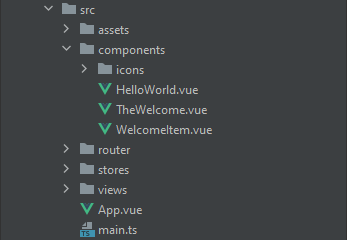
\includegraphics[width=0.4\textwidth]{img/vueFileStructure}
    \caption{Projektstruktur}
    \label{fig:vueProjektstruktur}
\end{figure}

\subsection*{Der virtuelle DOM}
Das Ändern des HTML-DOMs ist aufwändig und kann zu Performanceproblemen führen.
Für eine bessere Performance benutzt Vue.js einen virtuellen DOM.
Der virtuelle DOM ist eine Kopie des eigentlichen DOM.
Änderungen werden zunächst am virtuellen DOM vorgenommen.
Die Änderungen am virtuellen DOM ermöglicht es mehrere Änderungen zu bündeln,
bevor der reelle DOM angepasst wird. \cite[S. 10-11]{steyer2019} %TODO https://vuejs.org/guide/extras/rendering-mechanism.html#render-pipeline ?

\newpage

\subsection*{Model-View-ViewModel}
In Vue.js findet das MVVM-Pattern Anwendung.
Das sogenannte \emph{ViewModel} übernimmt die Vermittlung zwischen der View
und der Daten mit Businesslogik im Model.
Die Aufgabe des ViewModels übernimmt Vue.js.\cite[S. 43]{steyer2019}\footnote{In der Quelle ist die Rede von "MVVC". Aus dem Kontext ist klar, dass es sich um einen Tippfehler handelt und "MVVM" gemeint ist.}

\begin{figure}[H]
    \centering
    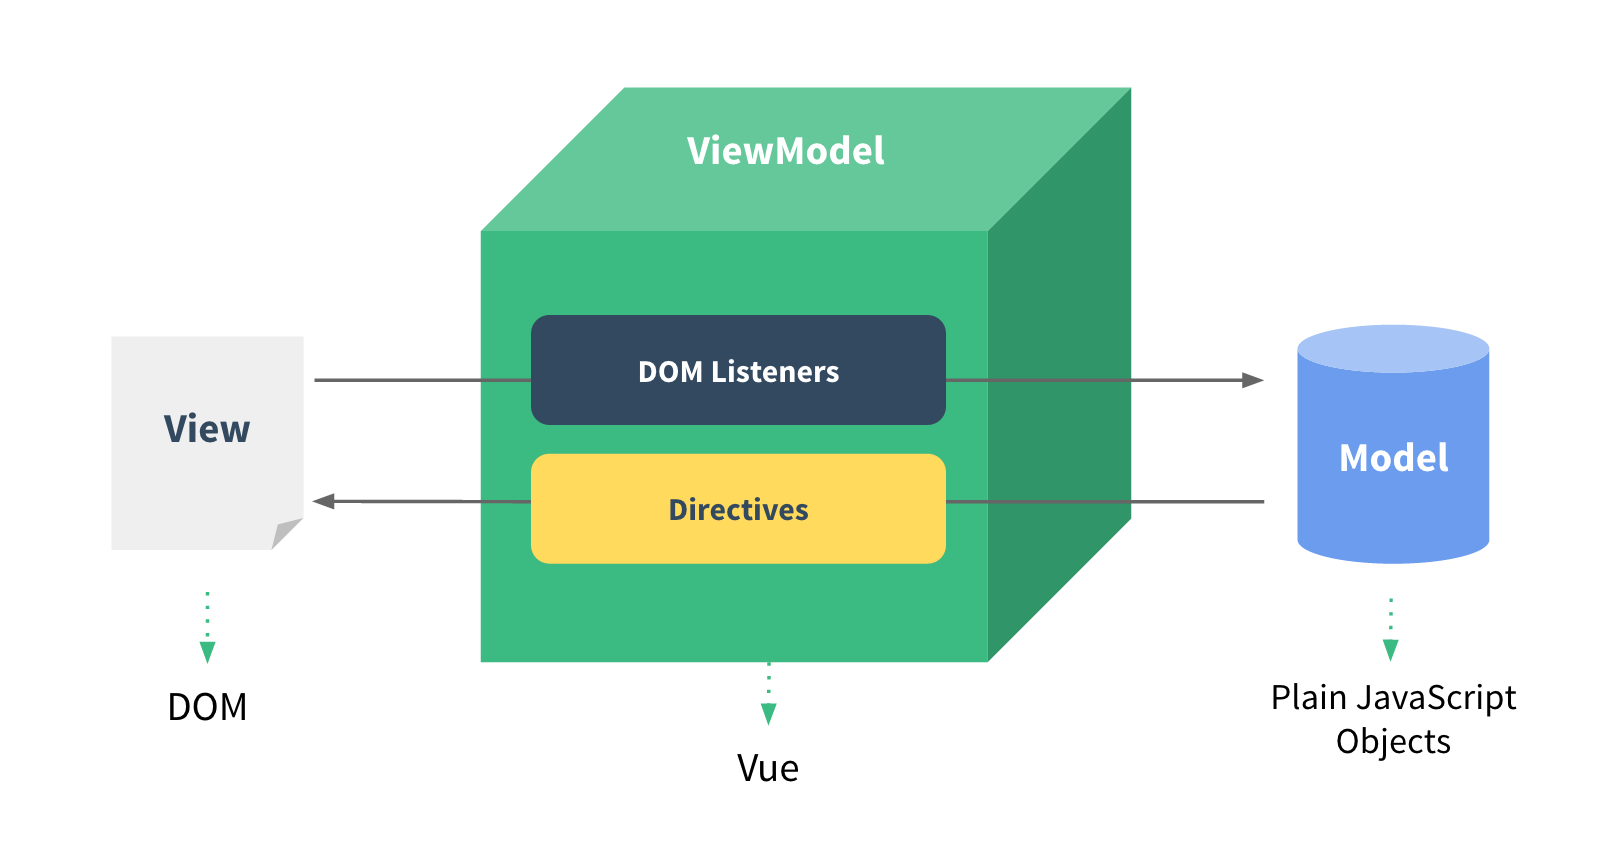
\includegraphics[width=0.8\textwidth]{img/mvvm}
    \caption{MVVM in Vue.js \cite{gettingStarted012}}
    \label{fig:mvvm}
\end{figure}

% ----------------------------------------------------------------------------